\documentclass{article}
\usepackage{graphicx}
\graphicspath{ {./images/} }
\title{Assigment 2}
\author{Muthya Narayanachary Akhil}
\date{January 29, 2024}

\begin{document}
\maketitle

\section*{Question 1}
\subsection*{Part a}
As stated in the question, we are required to calculate $C_{wire}$, which can be expressed by the following equation:

\begin{equation}
    C_{wire} = C_{pp} + C_{fringe}
\end{equation}

\subsubsection*{Calculating parallel plate capacitance}
Based on the lecture notes, this can be calculated in the following way:
\begin{equation}
    C_{pp} = \frac{38 * 10^{-18}}{1 * 10^{-12}} * 250 * 10^{-6} * 0.4 * 10^{-6} = 3800 * 10^{-18}F = 3800aF
\end{equation}

\subsubsection*{Calculating fringing capacitance}
This can be found in the following way:
\begin{equation}
    C_{fringe} = \frac{13 * 10^{-18}}{10^{-6}} * 250 * 10^{-6} = 3250 * 10^{-18} = 3250aF
\end{equation}

Since fringe capacitance needs to include for both the side walls, the value needs to be doubled, that is:

\begin{equation}
    C_{fringe} = 3250 * 2 = 6500aF
\end{equation}

\subsubsection*{Calculating the capacitance of the wire}
Based on (2) and (4), we can determine the capacitance of the wire in the following way:
\begin{equation}
    C_{wire} = C_{pp} + C_{fringe} = 3800 + 6500 = 10300aF = 10.3fF
\end{equation}

\subsection*{Part b}
The goal is to calculate the $R_{wire}$, given that the sheet metal resistance ($R_{0}$) is 0.08$\frac{\Omega}{sq}$.
The width is given to to be 0.4$\mu$m, hence the goal is to fit as many squares of this size into the available length.
This can be done in the following way:

\begin{equation}
    R_{wire} = 0.08 * \frac{250 * 10^{-6}}{0.4 * 10^{-6}} = 50\Omega
\end{equation}

\section*{Question 2}
\subsection*{Part a}
We are given that the current flowing through the wire is 4mA. Hence the IR drop can be given by:
\begin{equation}
    IR_{drop} = 4 * 10^{-3} * 50 = 0.2 V
\end{equation}

\subsection*{Part b}
We are given that the voltage source has an output impedance of 50$\Omega$, and requried to calculate the propagation delay ($t_{p}$).
Based off the lecture notes, we are aware the the $t_{p}$ is a function of resistance when on $R_{on}$ and the load capacitance $C_{L}$.

\begin{equation}
    t_{p} = f(R_{on} \cdot C_{L}) = 0.69 * R_{on} * C_{L}
\end{equation}
Since there is an impedance from the voltage source, $R_{on}$ can be calculated to be:
\begin{equation}
    R_{on} = R_{wire} + Z_{source} = 50 + 50 = 100\Omega
\end{equation}

Based on (5) and (9) we can compute the $t_{p}$ to be the following:
\begin{equation}
    t_{p} = 100 * 10.3 * 10^{-15} = 7.107 * 10^{-13} = 71.07ps
\end{equation}

\section*{Question 3}
\subsection*{Part a}
\subsubsection*{When $V_{in} = 0V$}
For the NMOS inverter shown above, when $V_{in}$ is 0V, the steady state $V_{out}$ is 1V.
This is because when $V_{in}$ is 0V, there is no curent at the gate, which doesnt lead to any holes appearing at the gate.
This means that there is no channel formed to faciliate electron flow, and hence the NMOS is turned off.
In short, this is because $V_{GS} < V_{TH}$ or the gate voltage is lesser than the threshold voltage.
This means that the $V_{DD}$ supply is used to charge the capacitor $C_{L}$, which would have the supply voltage across its terminals once it has been fully charged (ie at steady state).

\subsubsection*{When $V_{in} = 1V$}
However, when $V_{in}$ is 1V, we can notice that the gate voltage is greater than the threshold voltage and the NMOS is turned on.
When the NMOS can usually be considered to be a switch with a resistor. In this case the switch is turned on with a resistance of 10k$\Omega$.
This changes the nature of the circuit to be something like this:

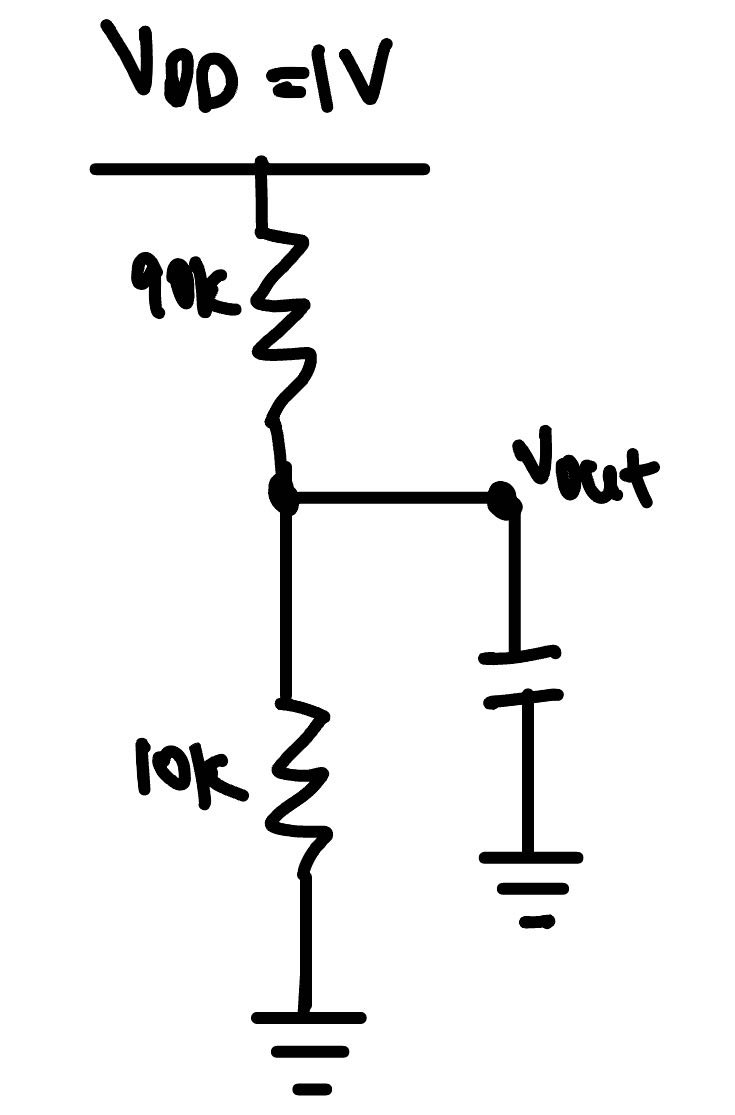
\includegraphics[scale = 0.2]{circuit2.jpg}

We can now use Ohms law for parallel circuits to calculate $V_{out}$ in the following manner:
\begin{equation}
    V_{out} = V_{in} * \frac{10k\Omega}{10k\Omega + 90k\Omega} = \frac{10}{100} = 0.1V
\end{equation}

\subsection*{Part b}
\subsubsection*{When $V_{in} = 0V$}
When $V_{in}$ = 0V, this means that the NMOS is turned off as $V_{GS}$ for the NMOS is less than the threshold voltage ($V_{THN}$).
However, in the case of the PMOS, this means that the gate voltage is negative in terms of the supply voltage. This means that electrons accumulate on the gate, which leads to holes creating a channel for current to flow from the source to the drain.
This ends up charging $C_{L}$, which ends up leading to $V_{out} = 1V$.

\subsubsection*{When $V_{in} = 1V$}
When $V_{in}$ = 1V, this means that the PMOS is turned off, as there is not enough potential difference to create a channel of holes. However the PMOS is turned off as $V_{GS} > V_{THN}$.
This leads to the curent flowing from the drain to the souce, and the capacitor is discharged, leading to the $V_{out} = 0V$.
\end{document}